\documentclass{article}
\usepackage[utf8]{inputenc}
\usepackage{graphicx}
\usepackage{geometry}
\usepackage{amsmath}
\usepackage{amsfonts}
\usepackage{float}
\usepackage{caption}
\usepackage{subcaption}
\usepackage{enumitem}

\geometry{left=25mm, top=25mm, right=25mm, bottom=25mm}

\title{PHY407 Lab 5}
\author{Pierino Zindel (1002429703) and Hayden Johnson (1002103537)}
\date{October 12, 2018}

\begin{document}

\maketitle

\noindent \textbf{Distribution of work:}

\section{Modeling space garbage (Newman 8.8)}

For this question we desire to model the trajectory of a ball bearing moving around a rod in space. We assume a negligible cross section of the rod and enough mass to avoid movement. Additionally, the trajectory of the ball bearing is taken to be in a plane perpendicular to the rod with $z=0$.

From part a) of exercise 8.8, the two second order odes that describe the orbit of the ball bearing are given as 

\begin{equation}
	\frac{d^2x}{dt^2} = f_x = -GM\frac{x}{r^2\sqrt{r^2 + L^2/4}}
	\label{eq:1}
\end{equation}
and 
\begin{equation}
	\frac{d^2y}{dt^2} = f_y = -GM\frac{y}{r^2\sqrt{r^2 + L^2/4}}
	\label{eq:2}
\end{equation}

where $r=\sqrt{x^2+y^2}$.

The two second-order odes were then converted to four first-order odes with 
\begin{equation}
	\frac{dv_x}{dt} = f_x 
\end{equation}
\begin{equation}
	\frac{dx}{dt} = v_x
\end{equation}
\begin{equation}
	\frac{dv_y}{dt} = f_y 
\end{equation}
\begin{equation}
	\frac{dy}{dt} = v_y 
\end{equation}

The system of equations was then solved using the 4th-order Runge-Kutta method with the initial conditions $x=1$, $y=0$, $v_x=0$, $v_y=1$; constant values $G=1$, $M=10$, $L=2$, and integrated over the interval $0<t<10$ with $1000$ steps. The resulting orbit trajectory of the ball bearing was then plotted and is shown in figure \ref{fig:q1_orbit}. We see that the resulting orbit is not a simple circular orbit but rather a precessing orbit as suggested in the textbook due to the rod having a non-spherical shape.


\begin{figure}[H]
	\centering
	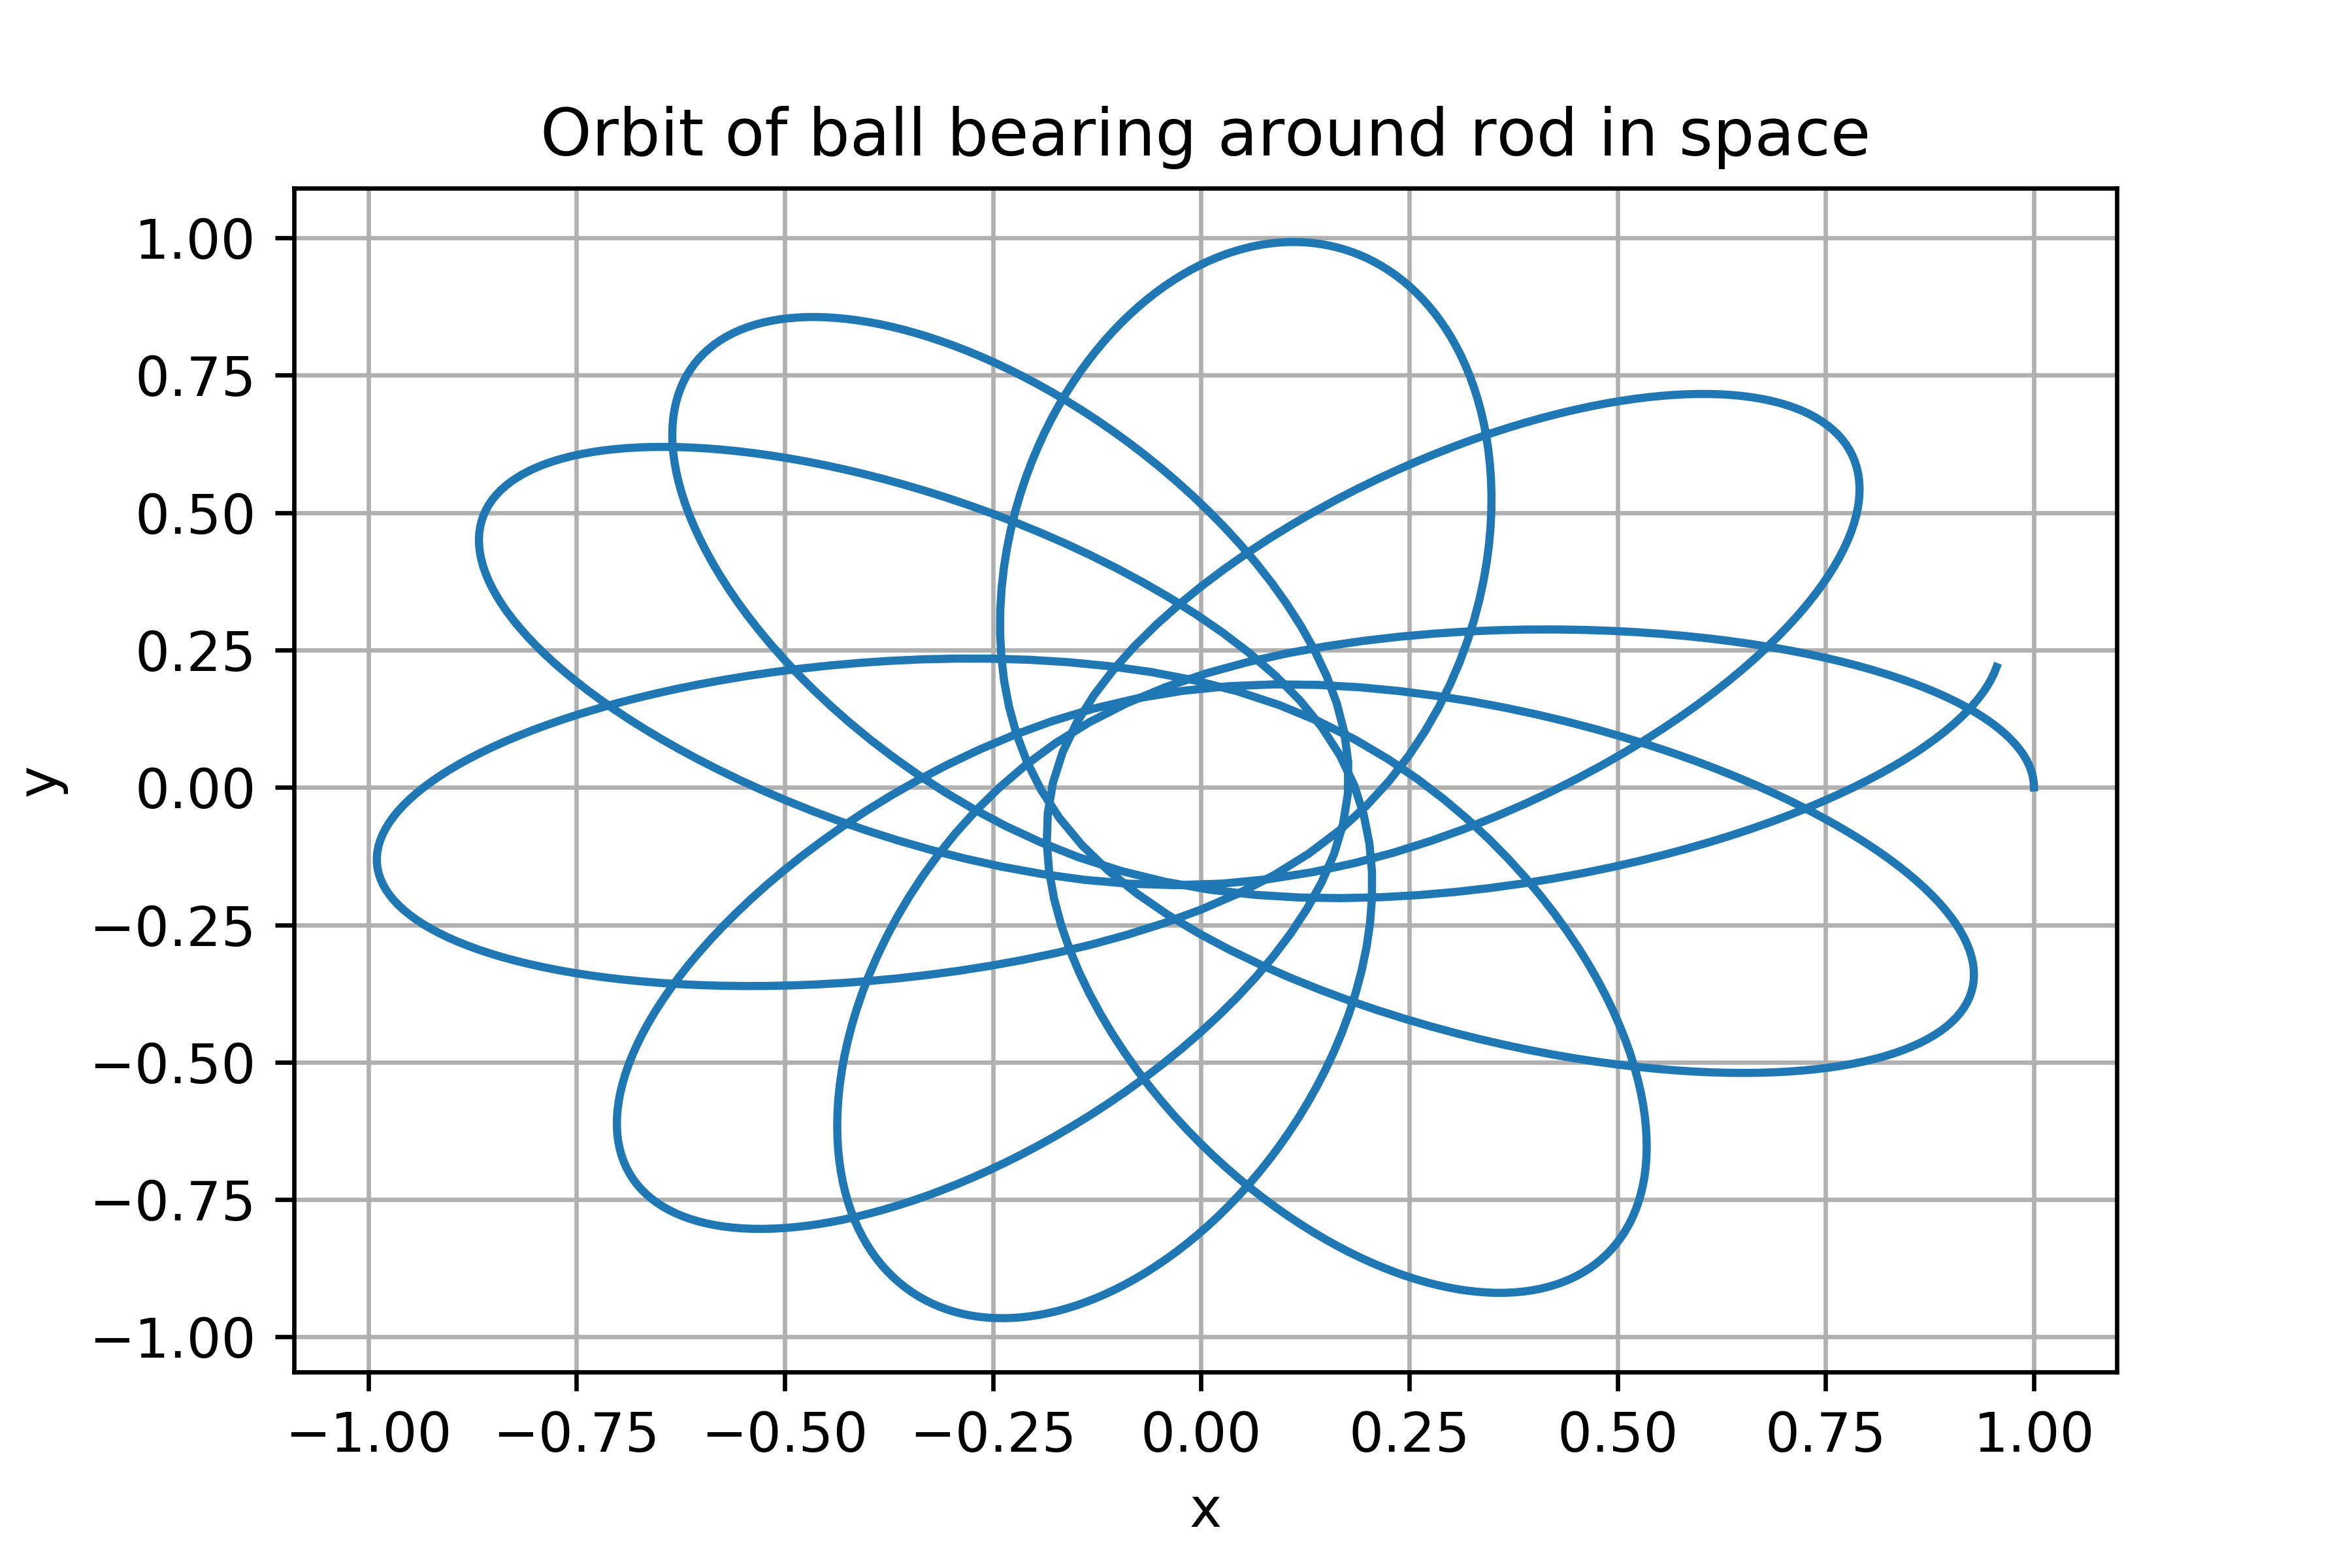
\includegraphics[width=0.8\textwidth]{../images/q1_orbit.png}
	\caption{Precessing orbit of a ball bearing around a rod, in a plane perpendicular to the rod. Equations of motion of the ball given by equations \ref{eq:1} and \ref{eq:2} with initial conditions of $(x,y,v_x,v_y)=(1,0,0,1)$.}
	\label{fig:q1_orbit}
\end{figure}

\section{Molecular Dynamics Simulation Part 1}

\subsection{Part b)}

We seek to write psuedocode, and then an actual program, to compute the trajectories of two particles interacting via the Lennard-Jones potential, and produce plots of the trajectories, for several different sets of initial conditions.

\subsubsection{Pseudocode}

\begin{enumerate}
	\item Define a function to compute the acceleration of each particle as a function of their positions
	\begin{enumerate}[label*=\arabic*]
		\item Compute the x and y distance between the particles
		\item Compute the square of the distance between the two particles
		\item Compute the scalar value of the force acting between the two particles (found by differentiating eq. 12 from the handout with respect to $r$)
		\item Compute the value of the x and y accelerations on each particle
	\end{enumerate}
	\item Input initial positions and velocities of particles
	\item 
\end{enumerate}

\end{document}
